\section{Distribution functions}\label{sec:df}

\subsection{General approach}\label{sec:df-general}

\galpy\ contains DF models to represent spherical and disky galactic components.
These DF models are constructed from a potential and a set of parameters,
they can be evaluated at phase-space points, integrated to obtain their moments 
(densities, mean velocities, and velocity dispersions), and they can be sampled.
On the backends, evaluation and the moments are differentiable for
every DF, sampling is differentiable wherever it is done by inverse
transformation, which is everywhere except for the many-position
velocity sampler of the quasi-isothermal disk DF and the samplers of
the two-dimensional disk DFs (\sectionname~\ref{sec:df-disk}), and
construction is differentiable for every DF whose construction is
itself a numerical computation---the spherical DFs obtained by
inverting a density, the King model, the quasi-isothermal disk DF,
whose table of guiding-center radii is then built on the backend, and
the stream models of \sectionname~\ref{sec:streams}. The parameters
of a DF, like those of a potential, can be given as backend arrays and
are then differentiated through everything that follows.

Every sampler in \galpy\ takes a \texttt{key=} argument:
\texttt{key=None} reproduces the previous behavior, drawing
from \numpy's global generator with the previous algorithm, while a
backend key selects the inverse-cumulative samplers of
\sectionname~\ref{sec:design-numerics} and returns backend arrays. For a
fixed key, the sample is then a smooth function of the DF's and the
potential's parameters, and its derivative is the pathwise, or
reparameterization, derivative: differentiating a statistic of the sample with respect to a
parameter gives an unbiased estimate of the derivative of the
expectation of that statistic. \figurename~\ref{fig:dfsample} shows an
explicit check that the pathwise derivative of a sample is the
derivative of the expectation, independently of any DF construction:
we differentiate a kernel estimate of the velocity dispersion over a
large fixed sample with respect to radius and compare with the
derivative of the Jeans equation; the two share no code and agree
within the Monte-Carlo noise. \figurename~\ref{fig:dfparam} then shows
the derivative of a sample through the construction of the DF, for an
Osipkov--Merritt DF of a Hernquist sphere constructed and sampled
inside a single compiled function of the scale radius: the derivative of
the sampled velocity dispersion with respect to the scale radius agrees
with the derivative of the Jeans-equation prediction to within the
Monte-Carlo noise, and with a finite difference of the same sample to
$10^{-7}$. The same figure shows the other kind of derivative of a DF's
construction, that of the King model's density profile with respect to
the dimensionless central potential $W_0$ at fixed mass and tidal
radius, which passes through the solution of the Poisson equation. In
eager mode, \galpy\ solves this ODE with \scipy\ and attaches the
derivative from the forward sensitivity equations, while under
compilation it solves the same ODE in the backend.

\begin{figure*}[t!]
  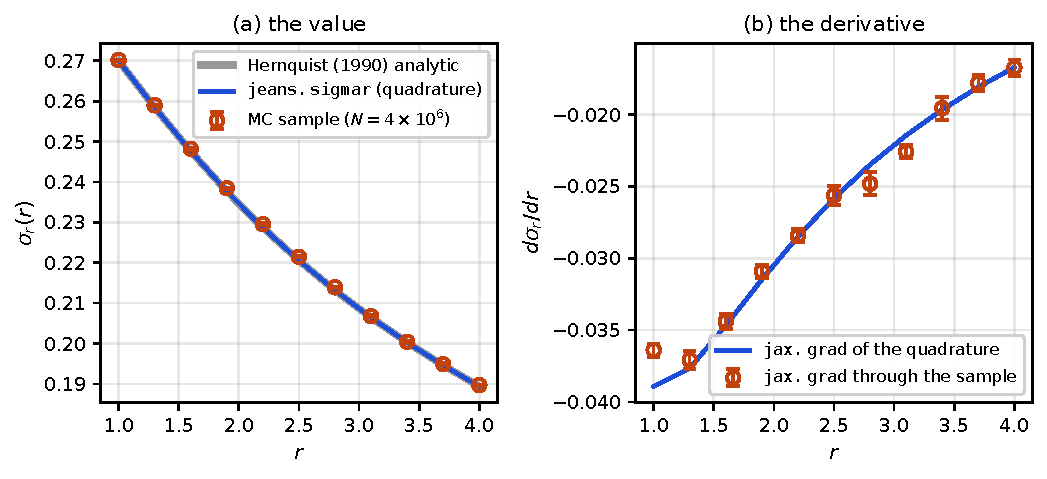
\includegraphics[width=\textwidth,clip=]{../figures/gD2_df_sample_autodiff/gD2_df_sample_autodiff.pdf}
  \caption{A derivative through a DF sample. Left: the radial velocity
    dispersion of the isotropic Hernquist DF from the analytic
    expression, from the Jeans equation by quadrature, and from a sample
    of $4\times10^6$ particles. Right: its derivative with respect to
    radius, from \texttt{jax.grad} of the Jeans quadrature and from
    \texttt{jax.grad} of a kernel estimator over the fixed sample, with
    error bars from eight sub-samples; the two agree to a median of
    $0.5\sigma$ of the Monte-Carlo noise, with the innermost point at
    $5\sigma$ from the bias of the kernel.}\label{fig:dfsample}
\end{figure*}

\begin{figure*}[t!]
  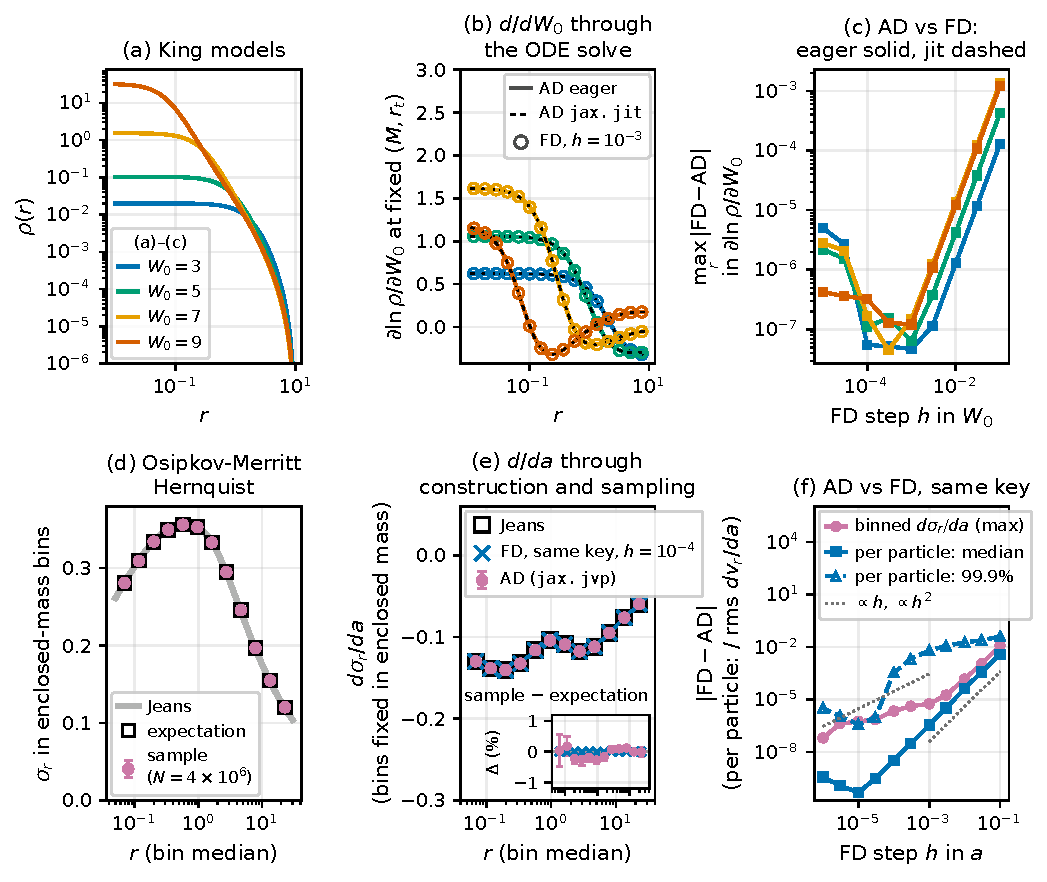
\includegraphics[width=\textwidth,clip=]{../figures/gD4_spherical_df_param/gD4_spherical_df_param.pdf}
  \caption{Derivatives through the construction and sampling of
    spherical DFs. Top row: (a) King models of unit mass and tidal radius
    $r_t=10$ for four values of $W_0$; (b) the derivative $\partial\ln\rho/\partial W_0$
    at fixed $(M,r_t)$ through the solution of the Poisson equation,
    eagerly with \scipy\ and under \texttt{jax.jit} with \diffrax, compared
    with a finite difference in which the model is rebuilt, and (c) the
    convergence of that finite difference onto the automatic derivative. 
    Bottom row: an Osipkov--Merritt DF of a Hernquist sphere with
    anisotropy radius $r_a=1.5$, constructed and sampled ($4\times10^6$
    particles) in one compiled function of the scale radius $a$; panel (d) shows that the
    sampled velocity dispersion matches the Jeans equation, (e) demonstrates that its
    derivative with respect to $a$ through construction and sampling
    matches both a finite difference of the same sample and the Jeans
    expectation within the Monte-Carlo noise, and panel (f) shows that the per-particle
    derivatives converge onto the automatic ones as $h$ and $h^2$.}\label{fig:dfparam}
\end{figure*}

\subsection{Spherical DFs}\label{sec:df-spherical}

The spherical DFs of \galpy---the Eddington inversion for isotropic
systems, the Osipkov--Merritt and constant-anisotropy inversions, the
King model, and the closed-form Hernquist and NFW DFs---share one
sampler, which draws radii by inverting the cumulative mass profile and
velocities by inverting a tabulated $p(v|r)$, and which on the backends
does both by interpolation in tables that are differentiable in their
knots. The inversions themselves, which are integrals of a derivative
of the density over the potential, use fixed-order Gauss--Legendre
quadrature in substituted variables and are differentiable through the
integrand, such that the DF can be differentiated with respect to the
parameters of the density and potential that it is built from. The
King model is the one DF whose \numpy\ result changed on purpose: its
Poisson equation is now solved to a relative tolerance of $10^{-10}$
rather than \scipy's default of $10^{-3}$, which left errors of order
$10^{-4}$ in its tables (\sectionname~\ref{sec:design-principles}). The
constant-anisotropy DF is the one place where \jax\ was already present
in \galpy, as an optional dependency for the fractional derivative in its
inversion; its construction is now much faster than it was, by about a
factor of four on \numpy\ and by orders of magnitude under
compilation, because the $f(E)$ inversion is a fixed-shape quadrature
that compiles well. As an example,
under \torch\ we obtain the derivative of a set of sampled radii with
respect to the scale radius of a Hernquist potential as
\begin{code}
a= torch.tensor(1.,dtype=torch.float64,
                requires_grad=True)
hp= HernquistPotential(amp=2.,a=a)
df= constantbetadf(pot=hp,beta=-0.2)
key= galpy.backend.random.key(7,backend='torch')
sam= df.sample(n=1000,key=key)
dr_da= torch.autograd.grad(sam.r().sum(),a)
\end{code}
and for a Hernquist sphere this derivative is $r_i/a$, which the sampler
reproduces to $10^{-13}$. Under \jax, construction, evaluation, and
sampling of these DFs run under \texttt{jax.jit}, and for the King
model so does the derivative with respect to $W_0$, as in for example
\begin{code}
def sigmar(W0):
    kdf= kingdf(W0=W0,M=2.3,rt=1.4)
    return kdf.sigmar(0.5)
dsig= jax.jit(jax.grad(sigmar)) # ODE by diffrax
dsig(3.)
\end{code}
A DF built from a density that is not the one generating the
potential is differentiable with respect to the parameters of both the
density and the potential; for example, with respect to those of the
density:
\begin{code}
def dispersion(a_tracer):
    hp= HernquistPotential(amp=0.1,a=a_tracer)
    df= eddingtondf(pot=NFWPotential(amp=1.,a=2.),
                    denspot=hp)
    return df.sigmar(1.)
jax.grad(dispersion)(0.7)
\end{code}
The closed-form DFs, including the analytic DFs of \citet{Evans1997}
for power-law spheres, and the energy derivative of their mass
profiles are likewise differentiable.

\subsection{Disk DFs}\label{sec:df-disk}

\galpy\ contains models for two-dimensional and three-dimensional disk DFs.
The two-dimensional axisymmetric disk DFs of \citet{Dehnen1999},
\citet{Shu1969}, and Schwarzschild
and their moments are evaluated with nested Gauss--Legendre quadrature
on the backends and are differentiable with respect to the parameters of
their surface-density and velocity-dispersion profiles; their samplers,
which draw by rejection, remain \numpy\ code, and we did not migrate
the corrections of these DFs for the difference between their input and
output profiles. \galpy\ also contains 
a two-dimensional non-axisymmetric disk DF that is a perturbation of a Dehnen DF by a
non-axisymmetric and/or time-dependent potential, which is evaluated by integrating orbits
backwards in time to an initial axisymmetric DF (in \texttt{galpy.df.evolveddiskdf}). 
The moments of
this evolved disk DF differentiate through that integration,
which on the backends is one vectorized in-backend solve over the
velocity grid rather than a loop. 

As a three-dimensional disk DF, \galpy\ implements the quasi-isothermal
DF of \citet{Binney2010,BinneyMcMillan2011}, in the form used by
\citet{BovyRix2013},
which is a function of the actions and is evaluated by first computing the actions with 
\texttt{actionAngleStaeckel} and then evaluating the DF.  The quasi-isothermal DF is now 
evaluated and its moments computed on the backends,
differentiably with respect to the parameters of the potential and the
DF's scale lengths, and its velocity sampler at a given position draws
by inverse transformation on a three-dimensional velocity mesh, such
that a sample drawn with a fixed key is a differentiable function of the
DF's parameters;
this sampler replaced a rejection sampler on the \numpy\ path as well,
which is one of the two places where the \numpy\ draws changed (the
distribution is the same, the particular draws are not). In code this looks as follows:
\begin{code}
qdf= quasiisothermaldf(1./3.,0.2,0.1,1.,1.,
                       pot=MWPotential2014,aA=aAS)
vs= qdf.sampleV(0.9,0.05,n=10**4,
                key=grandom.key(0,backend='jax'))
sigma_R= jnp.std(vs[:,0])
\end{code}
Its construction tabulates the guiding-center radius as a function of
angular momentum, which is built on the backend when the potential or a
scale length carries a backend parameter, such that the DF and its
moments are differentiable through the construction. Its interpolated
velocity sampler, which samples many positions at once, is a rejection
sampler with \numpy\ proposals that runs on the backends, with its
shrinking arrays padded to fixed sizes, but is not differentiable.

\subsection{Speed}\label{sec:df-speed}

Sampling is where the backends change what is practical, as is clear
from \figurename~\ref{fig:dfspeed}, which displays the time to draw $N$
particles from four spherical DFs. On the CPU, eager \jax\ and \torch\ are slower
than \numpy\ for small samples, because every one of the hundreds of
array operations in a draw is dispatched separately and each costs a few
to tens of microseconds, and they catch up only at $N\approx10^4$;
compiled \jax\ is faster than \numpy\ at every size, by a factor of
1.5 to 6 at $N=10^7$ on one core, because the compiler fuses the
hundreds of array operations of a draw into a few loops, where \numpy\
executes each separately and writes its intermediate results to
memory. On a GPU the sample of $10^7$ particles takes
tens of milliseconds on the consumer card and a few milliseconds on the
H100, two to nearly four orders of magnitude faster than \numpy\ on
one core. The lower panel
shows the cost of constructing a DF, which for the inversions is
dominated by the $f(E)$ integral: more than a minute on \numpy\ for the
constant-anisotropy DF, a fraction of a second once compiled, with the
compilation itself costing seconds and paid once.

\begin{figure*}[t!]
  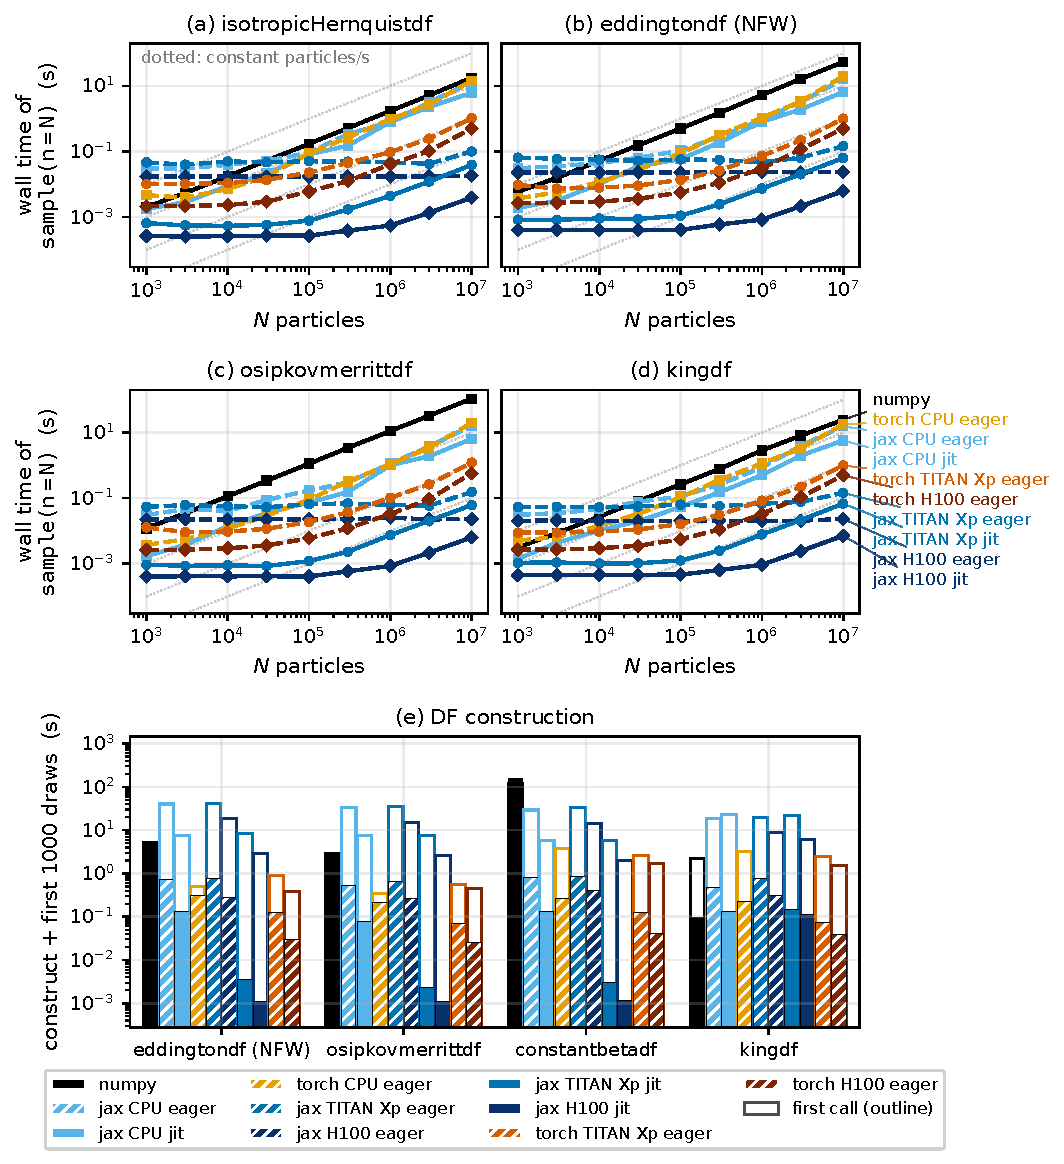
\includegraphics[width=\textwidth,clip=]{../figures/gD3_spherical_df_speed/gD3_spherical_df_speed.pdf}
  \caption{Speed of sampling and constructing spherical DFs. Top: wall
    time of \texttt{sample(n=N)} for the isotropic Hernquist DF, the
    Eddington inversion of an NFW profile, an Osipkov--Merritt DF, and a
    King model, on \numpy\ and on the backends on the CPU, the TITAN~Xp,
    and the H100; solid lines are compiled, dashed eager. Bottom: time to
    construct each DF and draw a first thousand particles, warm (filled)
    and including compilation on the first call in a fresh process
    (outline); hatched bars are eager. All CPU series use one core. Compiling with \texttt{jax.jit} or
    running on a GPU makes sampling much faster than with \numpy, by two
    to nearly four orders of magnitude on a GPU for large samples.}\label{fig:dfspeed}
\end{figure*}
